\documentclass[10pt]{beamer}

\usefonttheme{serif}

\usepackage{amsmath}
\usepackage{amssymb}
\usepackage{graphicx}

\usetheme[pageofpages=of,% String used between the current page and the
                         % total page count.
          bullet=circle,% Use circles instead of squares for bullets.
          titleline=true,% Show a line below the frame title.
          alternativetitlepage=true
          ]{Torino}

%\usecolortheme{nouvelle}

\title[Epidemic Forecasting]
{Epidemic Forecasting}
\subtitle
{Review of the state of the art}
\author{Dexter Barrows}
\institute[McMaster University]
{
  Department of Mathematics and Statistics\\
  McMaster University
}
\date[Presentation]
{March 19 2015}


\begin{document}

		\begin{frame}[t,plain]
			\maketitle
		\end{frame}

		\begin{frame}{Outline}
			\setbeamercolor{section in toc}{fg=black}
			\setbeamercolor{subsection in toc}{fg=chameleongreen3}
		  	\tableofcontents
		\end{frame}


	\section{Techniques}

		\begin{frame}[allowframebreaks]{ARIMA}
			\begin{itemize}
				\item {\bf A}uto{\bf R}egressive {\bf I}ntegrated {\bf M}oving {\bf A}verage
				\item Depends {\bf only} on the data
				\item 3-parameter process $ARIMA(p,d,q)$, indicating order of
					\begin{itemize}
						\item p - autoregressive
						\item d - integrated
						\item q - moving average
					\end{itemize}
					components
				\item General form
					\begin{equation*}
						\left( 1 - \sum_{i=1}^{p} \varphi_i L^i \right) (1-L)^d X_t = \left( 1 + \sum_{i=1}^{q} \theta_i L^i \right) \varepsilon_t
					\end{equation*}
					where $X_t$ is the time series being considered\\
					{\it (Should I define the other variables/parameters/operators?)}

				\framebreak
				\item Forecasting using $ARIMA$
					\begin{enumerate}
						\item Consider the process $Y_t = (1-L)^d X_t$ which is non-stationary
						\item Then the wide-sense stationary process
							\begin{equation*}
								\left( 1 - \sum_{i=1}^{p} \varphi_i L^i \right) Y_t = \left( 1 + \sum_{i=1}^{q} \theta_i L^i \right) \varepsilon_t
							\end{equation*}
							can be used to forecast using auto regressive (n-step ahead) forecasting once the parameters have been estimated, using
							\begin{equation*}
								Y_{t+1} = c + \sum_{i=0}^{p-1} \varphi_{i+1} Y_{t-i}
							\end{equation*}
					\end{enumerate}
			\end{itemize}
		\end{frame}

		\begin{frame}{SARIMA}
			\begin{itemize}
				\item Adaptation of $ARIMA$ used to capture seasonal effects
				\item Usually expressed as $SARIMA (p,d,q) \times (P,D,Q)_s$, where $P,D$ and $Q$ indicate the order of the seasonal autoregressive, integrated, and moving average components
				\item A combination of autocorrelation functions ($ACF$) and partial autocorrelation functions ($PACF$) are used to determine optimal non-seasonal and seasonal orders
			\end{itemize}
		\end{frame}

		\begin{frame}{S-mapping (1)}
			\begin{itemize}
				\item Sequentially locally weighted global linear maps (S-map)
				\item Procedure
				\begin{enumerate}
					\item Construct a ``library'' of consecutive time lag vectors $\{x_i\}$ of length $E$ and corresponding forward trajectories $\{y_i\}$
					\item Choose a state $x_t$ from which you wish to forecast the next system state $y_t$
					\item The estimation $\hat{y_t}$ is evaluated using
						\begin{equation*}
							\hat{y_t} = \sum_{j=0}^E c_t(j)x_t(j).
						\end{equation*}
						Here $c$ is obtained by solving the system $b=Ac$ where
						\begin{equation*}
							\begin{array}{rl}
								b(i) 	& = w(||x_i-x_t||) y_i \\
								A(i,j) 	& = w(||x_i-x_t||) x_i(j)
							\end{array}
						\end{equation*}
						where the weights are a function of Euclidean distance
						\begin{equation*}
							w(d) = e^{ \frac{-\theta d}{\bar{d}} }
						\end{equation*}
				\end{enumerate}
			\end{itemize}
		\end{frame}

		\begin{frame}{Simplex projection}
			\begin{center}
				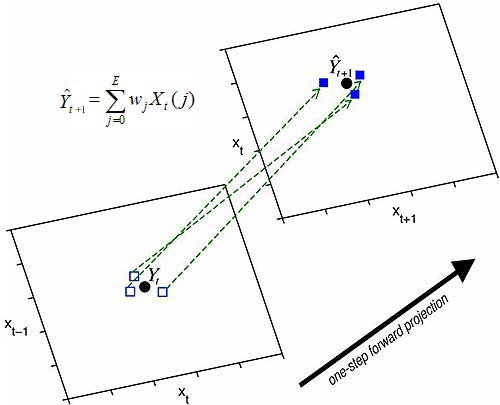
\includegraphics[width=\textwidth,height=0.75\textheight,keepaspectratio=true]{images/simplex.jpg}
				\\
				{\it \small \url{http://simplex.ucsd.edu/} }
			\end{center}
		\end{frame}

		\begin{frame}{S-mapping}
			\begin{center}
				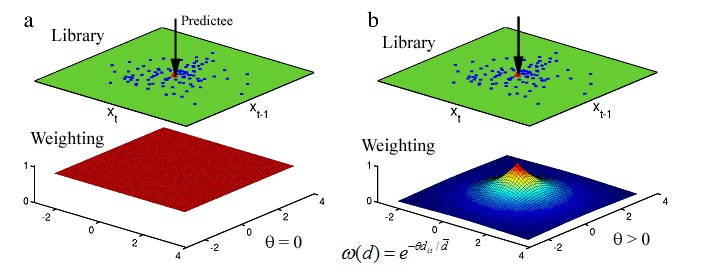
\includegraphics[width=\textwidth,height=0.75\textheight,keepaspectratio=true]{images/smap.jpg}
				\\
				{\it \small \url{http://simplex.ucsd.edu/} }
			\end{center}
		\end{frame}

		\begin{frame}{Kalman filter}
			\begin{itemize}
				\item Predictive method that operates on noisy data to produce optimal estimate of next system state
				\item Designed to operate on linear models
				\item Uses a model of expected system behaviour (for example a system of ODEs) to help with prediction
				\item Model (common simplified form)
					\begin{equation*}
						\begin{array}{rl}
							x_t & = F x_{t-1} + w_t \\
							z_t & = H x_t + v_t
						\end{array}
					\end{equation*}
					where the $x_t$ is the state being predicted, and the noise components $w_t$ and $v_t$ are drawn from covariance matrices updated at each iteration
				\item These equations form the basis of a prediction / measurement update cycle\\
					{\it (Should I include the equations for the cycle?)}
			\end{itemize}
		\end{frame}

		\begin{frame}{Kalman filter extensions}
			\begin{itemize}
				\item Extended Kalman filter ($EKF$)
					\begin{itemize}
					 	\item Nonlinear version of the standard Kalman filter
					 	\item Linearises about the estimate of current mean and covariance
					\end{itemize}
				\item Ensemble Kalman filter ($EnKF$) 
					\begin{itemize}
						\item Uses a cohort of ensemble members, and uses the sample mean and covariance instead of a covariance matrix (faster)
						\item Still assumes all distributions are Gaussian
						\item Designed for problems with a large number of parameters
					\end{itemize}
				\item Ensemble Adjustment Kalman filter ($EAKF$) 
					\begin{itemize}
						\item Combination of $EKF$ and $EnKF$ 
						\begin{itemize}
							\item Linearises about the estimate of current mean and covariance
							\item Also uses ensemble members to avoid use of covariance matrices
						\end{itemize}
					\end{itemize}
			\end{itemize}
		\end{frame}

		\begin{frame}{Particle filter}
			\begin{itemize}
				\item Uses a set of particles to attempt to infer the effect a hidden Markov Model given observations of only some variables in a system; similar to $EnKF$
				\item Makes no assumption about the distributions involved in the system
				\item General structure of the basic particle filter with Sequential importance resampling
				\begin{itemize}
					\item Each of the $P$ particles at time $t$ consists of a weight-state pair $(w_t^{(i)},x_t^{(i)})$, such that $\sum\limits_{i=1}^{P} w_t^{(i)} = 1$
					\item Next system state (forecast) is given by the weighted average $\hat{x_t} = \sum\limits_{i=1}^{P} w_{t-1}^{(i)} f(x_{t-1}^{(i)})$
					\item After forecast, a new observation $x_t$ is assimilated and weights are recalculated based on how accurate the individual projections were
				\end{itemize}
				\item Degeneracy occurs when a single particle accumulates almost all weight, leaving the rest of the particles with weighting near or at 0
				\begin{itemize}
					\item Avoided via resampling at each iteration
				\end{itemize}
				

			\end{itemize}
		\end{frame}

		\begin{frame}{Particle filter extensions}
			\begin{itemize}
				\item Maximum likelihood via iterated filtering ($MIF$)
					\begin{itemize}
					 	\item Uses multiple rounds of particle filtering, where each round is used to inform the initial distribution of particles in the parameter space for the next round
					 	\item Each round pushes the parameter estimates further toward maximum likelihood
					\end{itemize}
				\item Particle Markov chain Monte Carlo ($pMCMC$)
					\begin{itemize}
					 	\item Uses an MCMC method (typically the Metropolis-Hastings algorithm) to constrain model parameters, and a particle filter between each MCMC iteration
					 	\item Each round of particle filtering uses the set of parameters proposed by the MCMC iteration
					\end{itemize}

			\end{itemize}
		\end{frame}


	\section{Underlying dynamics}

		\begin{frame}[allowframebreaks]{SIR-based model formulations}

			\begin{itemize}
				\item Extensively used model in epidemiology
				\item Division into classes: {\bf S}usceptible-{\bf I}nfected-{\bf R}emoved
				\item Transition between states
					\begin{equation*}
						\begin{array}{rl}
							\frac{dS}{dt} & = - \frac{\beta I S}{N} \\
							\frac{dI}{dt} & = \frac{\beta I S}{N} - \gamma  \\
							\frac{dR}{dt} & = \gamma I
						\end{array}
					\end{equation*}
				\item Many extensions exist
				\begin{itemize}
					\item Additional classes
					\item Additional mechanistic terms
				\end{itemize}
			\end{itemize}

			\framebreak
			\begin{center}
				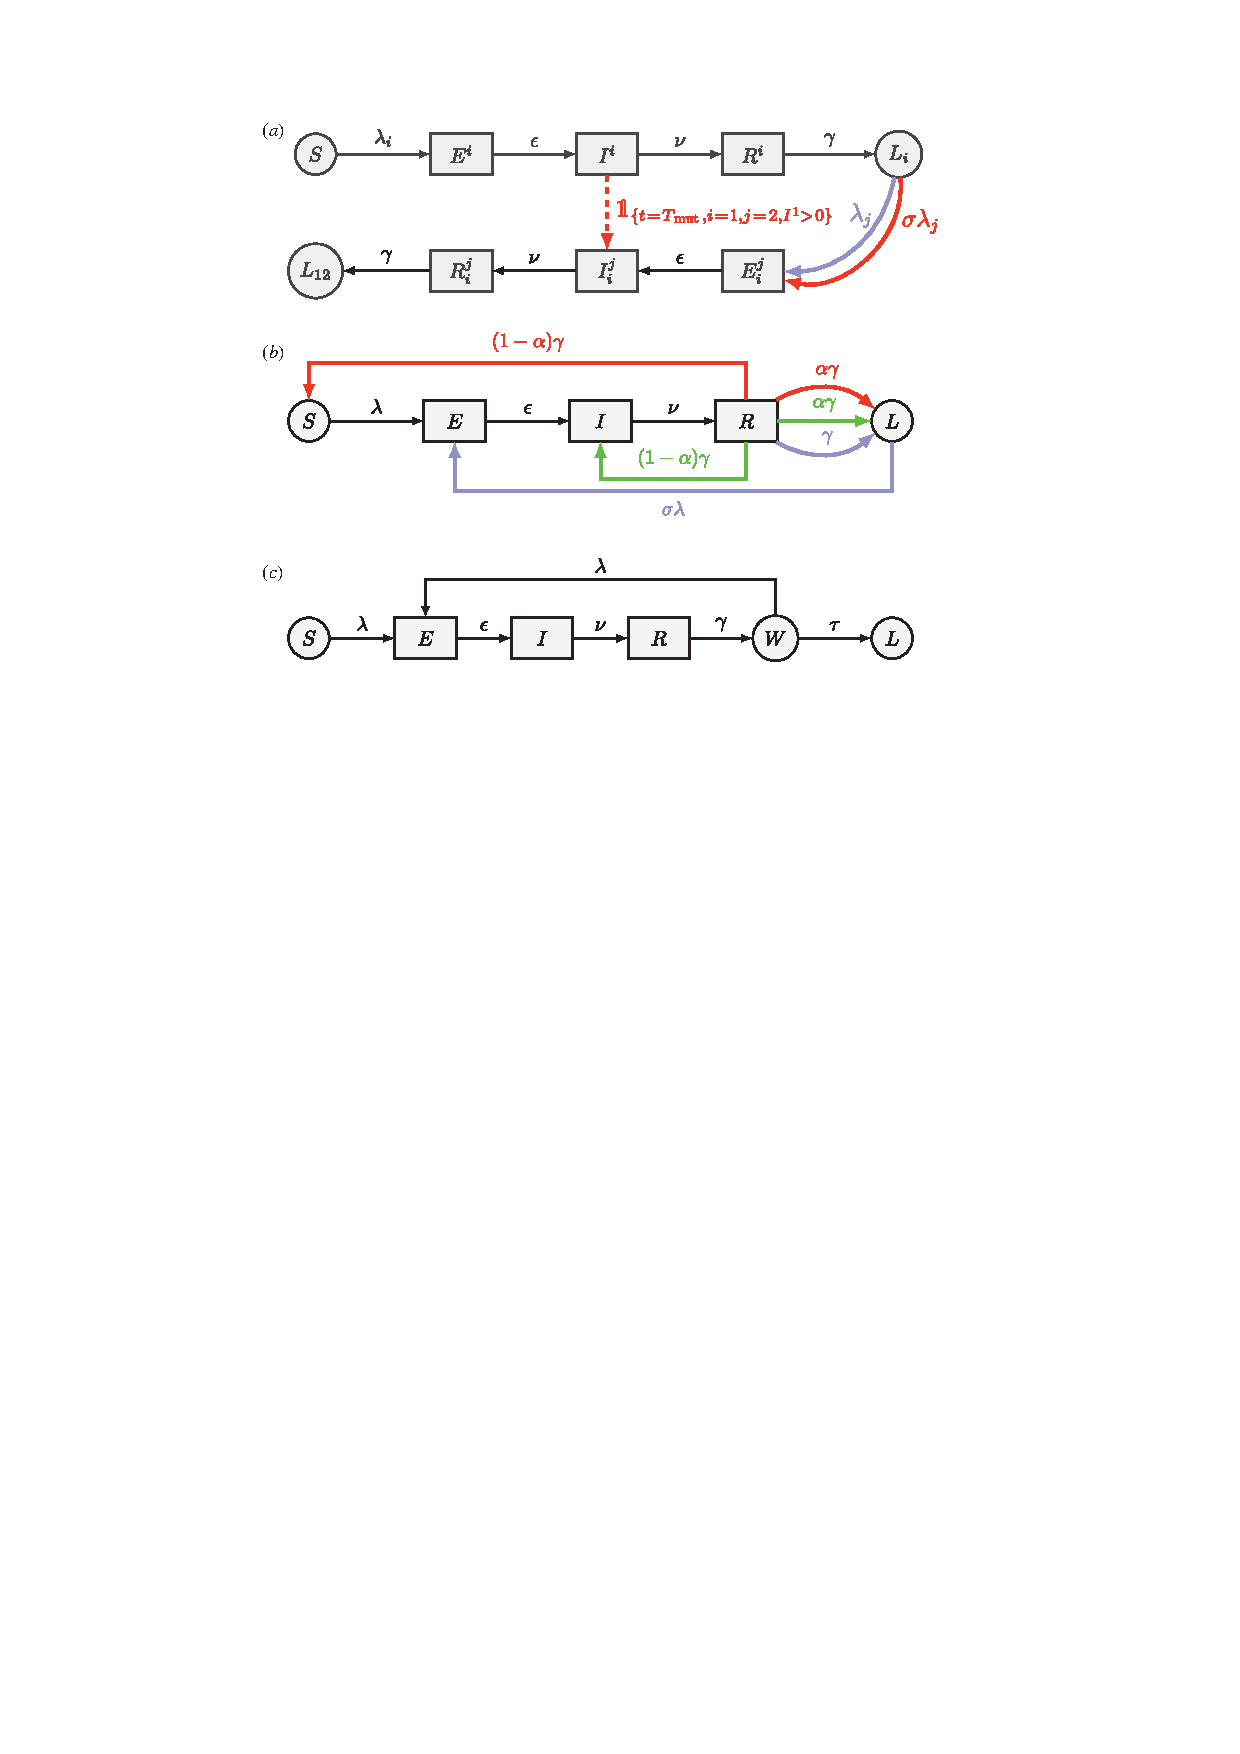
\includegraphics[width=\textwidth,height=0.75\textheight,keepaspectratio=true]{images/seir_variations.pdf}
				\\
				{\it \small Camacho et al, 2011}
			\end{center}

		\end{frame}

		\begin{frame}{Parameter fitting}
			\begin{itemize}
				\item SIR-based models may require many parameters to be estimated
				\item Overfitting a particular problem - can reduce forecasting ability
				\item More model complexity $=$ longer time series required
				\item Iterated filtering methods can estimate parameters in addition to producing forecasts
			\end{itemize}
		\end{frame}

		\begin{frame}
			\frametitle{AIC}
			\begin{itemize}
				\item {\bf A}kaike {\bf I}nformation {\bf C}riterion
				\item A way to compare models of different complexities
			\end{itemize}
		\end{frame}


	\section{Data assimilation}

		\begin{frame}
			\frametitle{Incidence data}
		\end{frame}

		\begin{frame}
			\frametitle{ENSO}
		\end{frame}

		\begin{frame}
			\frametitle{Seasonal trends}
		\end{frame}

	\section{Measuring prediction accuracy}

		\begin{frame}
			\begin{itemize}
				\item Peak timing / intensity
				\item Magnitude
				\item Duration
				\item Daily / weekly Activity
				\item RMSE
				\item ROC curves
			\end{itemize}
		\end{frame}


		
		
\end{document}
